% 2019-04-10

\documentclass[10pt]{article}
\usepackage[T1]{fontenc}
\usepackage{amssymb}
\usepackage{amsmath}
\usepackage{graphicx}
% \begin{figure}[h]
% \centering
% \includegraphics[width=6.5in]{folder/photo.png}
% \caption{}
% \label{}
% \end{figure}



\usepackage{tikz}
\usetikzlibrary{arrows}
\usepackage{subfigure}
\usepackage{stackrel}
\usepackage{blindtext}

\usepackage{biblatex}
\addbibresource{library.bib}

\oddsidemargin=0.15in
\evensidemargin=0.15in
\topmargin=-.5in
\textheight=9in
\textwidth=6.25in

\usepackage[colorlinks=true,breaklinks,pdfpagemode=none,linkcolor=blue,citecolor=blue]{hyperref}

\usepackage{enumerate}
% \vspace{-6pt}
% \begin{itemize}
%     \setlength{\itemsep}{0pt}%
%     \setlength{\parskip}{0pt}%
%     \item Item 1
%     \item Item 2
%         \begin{itemize}
%             \setlength{\itemsep}{0pt}%
%             \setlength{\parskip}{0pt}%
%             \item Sublist Item 1
%             \item Sublist Item 2
%         \end{itemize}
%         \item Item 3
% \end{itemize}
% \vspace{-6pt}


\usepackage{enumitem}
\setlist{itemsep=0mm}

\usepackage{amsmath,amsfonts,amssymb,bm}


\begin{document}

   \noindent
   \begin{center}

   \hrulefill
   
   \vspace{5pt}
   
   \makebox[\textwidth]{ {\bf Energy Systems Analysis} \hfill  A.D. Smith 2019}
   \vspace{0pt}
   
   {\Large \hfill  Lecture 32.  
Distributed Thermal Energy Storage
}
   \vspace{5pt}
   
  
   \hrulefill
   \end{center}

 {\color{darkgray}{\center{ \small{      ``Support for the R&D of new storage materials, as well as policy measures and investment
incentives for TES integration in buildings, for industrial applications, and for variable renewable
power generation, is essential if [TES] deployment is to be fostered.''
\\%[3pt]
\rightline{{\rm --- Sarbu and Sebarchievici  \cite{Sarbu2018-yg}}}}}}}




\section{What is distributed thermal energy storage?}

Thermal energy storage (TES) (also simply called thermal storage) has been commonly used at the single-building level and the district level for decades, if not centuries. While it has received increasing attention and research interest over the last three decades or so, it can be broadly defined as a storage device that stores heat (or the absence of heat) so that thermal energy can be delivered (or removed) at a later time. This includes familiar devices that don't necessarily spring to mind with 'energy storage' such as your home water heater (unless it's tankless).\\

In a recent review, Sarbu and Sebarchievici formally describe it as follows:

\begin{quote}
    Thermal energy storage (TES) is a technology that stocks thermal energy by heating or
cooling a storage medium so that the stored energy can be used at a later time for heating and cooling
applications and power generation. TES systems are used particularly in buildings and in industrial
processes. \cite{Sarbu2018-yg}
\end{quote}

They also provide a figure summarizing the types of thermal storage that can be used in conjunction with solar energy, reproduced in Figure \ref{types}.

\begin{figure}[h]
\centering
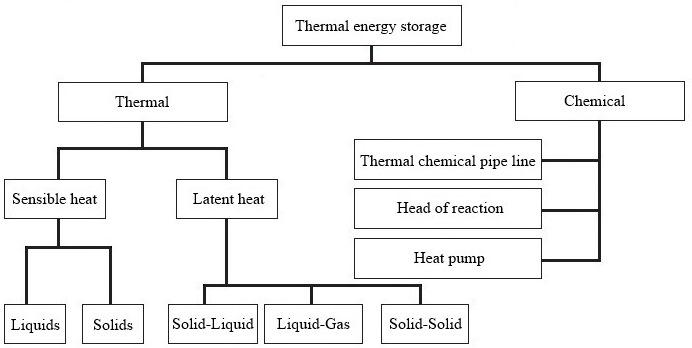
\includegraphics[width=5.5in]{extras32/types.jpg}
\caption{Types of solar thermal energy storage \cite{Sarbu2018-yg}}
\label{types}
\end{figure}


\section{Heat Storage}

As with electrical energy storage, the primary function of thermal energy storage is to shift the use of thermal energy in time, with the goal of storing as much energy as possible in the given volume of the storage device.

A TES system that ``stores heat'' (a common phrasing that is not technically correct, as we know from our studies in thermodynamics that the word 'heat' refers to energy in transit) can serve the needs of a building for providing space heating or hot water, or process heat in larger commercial or industrial facilities. 



\subsection{Sensible heat storage}

Sensible thermal energy storage, as the name suggests, does not involve phase change for the working material. The working material could be something like rock or water. Your water heater is an example of sensible heat storage---you expect that the water will remain liquid throughout the process of being heated and leaving the water tank at a later time.

Key characteristics associated with TES are the specific heat of the material $c_p$ and the temperature difference $\Delta T$ between the beginning and end of the storage period, or between the temperature of the storage medium and the temperature of the ``load'' (medium to which heat is being transferred). Its capacity would be the amount of stored thermal energy in BTU, kWh, or J. 

As with battery modeling, we have a variety of options for how much detail we need to represent for a TES system in the context of a larger facility with multiple energy systems. A simple 1-D computational model can provide relevant operational parameters including heat exchanger temperatures values, and stored water temperatures as functions of time at particular locations within the tank \cite{Aowabin2}.


\subsection{Latent heat storage}

Latent thermal energy storage involves phase change (although a latent TES system will often incorporate some sensible heat storage as well). The working material could be something like a salt hydrate or water. There is a significant amount of latent energy associated with boiling and condensing of water, i.e. the latent heat of vaporization, but usually when people discuss latent TES that is water-based they are talking about cold thermal storage (Section \ref{coldTES}). A key characteristic here is the phase change enthalpy difference $\Delta h$.

There has been increased interest over the past decade or so in developing phase-change materials (PCM) that have ideal characteristics for specific thermal storage applications, including embedding PCMs in the walls of a building to reduce temperature swings and thus reduce the need for heating and cooling (i.e. strategically increasing the thermal mass of the building). This can include everyday materials like polyethylene glycol or naphthalene, but can also include a variety of complex advanced engineered materials with nano-enhancement \cite{Shah2018-hl}.

\subsection{With combined heat and power systems}

Although the benefits are highly dependent on the building's loads and the sizing of the energy systems, adding TES to a combined heat and power (CHP) system in a commercial facility can provide reductions in operational cost, primary energy consumption, and carbon dioxide emissions \cite{Smith2013-xo}. The general setup is illustrated in the schematic in Figure \ref{CHP-TES}. The thermal storage tank acts as a buffer between the heat recovery system that captures the ``waste'' heat from the power generation unit, and stores that energy (limited by the thermal capacity of the tank) until a later time when the thermal energy is needed by the building. This can reduce the amount of time that the building's boiler needs to operate (and thus the amount of fuel that it needs to burn, the frequency of maintenance required, etc.) and, in special cases, may remove the requirement for an auxiliary boiler entirely. 


\begin{figure}[h]
\centering
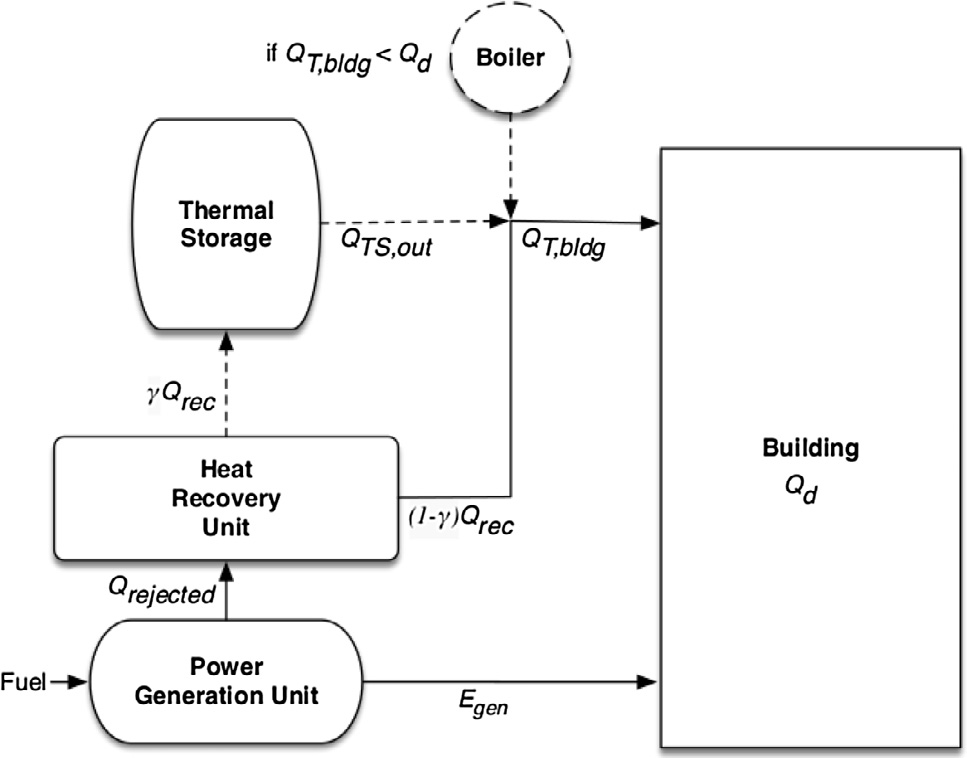
\includegraphics[width=4.5in]{extras32/CHP-tes.jpg}
\caption{CHP-TES system schematic \cite{Rahman2018-yc}}
\label{CHP-TES}
\end{figure}


\section{Cold Storage}
\label{coldTES}

With cold thermal energy storage (CTES), we are still shifting the use of thermal energy in time, but we are talking about transferring heat \textit{out} of a given medium so that its temperature is below ambient, and then using that medium to cool (i.e. accept heat from) some other medium at a later time.

Cold storage in buildings or groups of buildings usually means chilling ice or water and using the medium for cooling during a time of peak demand---or, more accurately from the building operator's perspective, a time of peak \textit{pricing}. This is a type of load shifting, or demand-side energy management. This may also be done to reduce the amount of needed chiller capacity, but because the CTES system will have costs associated with it, it's more likely that CTES will be installed when there is also a financial incentive to shift the load in time. If the chiller's load factor would be extremely low, the reduction in capacity might be worth it on its own. Careful engineering analysis of the total first costs and the operating savings over the system's lifetime is needed \cite{McQuiston2005-oo}.
 
 \subsection{Chilled water storage}
 
 Chilled water storage will require a large volume for the storage tank, and may benefit from economies of scale as the storage volume increases, although the space available at the site may be limited. Chilled water storage may be a first option to consider for an institutional campus where the demand for chilled water is large and predictable, and there is space available to dedicate to a chilled water facility.
 
 \subsection{Ice storage}
 
 Ice storage will require less volume due to the significant amount of latent energy associated with freezing and melting of water, i.e. the latent heat of fusion. However, ice storage will require more insulation than chilled water storage because its $H_2O$ is at a lower temperature, and chillers will be less efficient as the temperature is reduced. Ice storage may be a first option to consider for an small-to-medium sized CTES system, such as for a single commercial building.


% license
\bigskip

\noindent
\texttt{\footnotesize RESTRICTED PUBLIC LICENSE --- READ BEFORE SHARING. This is a draft version made available by Amanda D. Smith under a Creative Commons Attribution-NonCommercial-ShareAlike license. 
\href{https://creativecommons.org/licenses/by-nc-sa/4.0/}{CC BY-NC-SA 4.0}}


\printbibliography

\end{document}